% Options for packages loaded elsewhere
\PassOptionsToPackage{unicode}{hyperref}
\PassOptionsToPackage{hyphens}{url}
\documentclass[
  11pt,
]{article}
\usepackage{xcolor}
\usepackage[margin=0.8in]{geometry}
\usepackage{amsmath,amssymb}
\setcounter{secnumdepth}{-\maxdimen} % remove section numbering
\usepackage{iftex}
\ifPDFTeX
  \usepackage[T1]{fontenc}
  \usepackage[utf8]{inputenc}
  \usepackage{textcomp} % provide euro and other symbols
\else % if luatex or xetex
  \usepackage{unicode-math} % this also loads fontspec
  \defaultfontfeatures{Scale=MatchLowercase}
  \defaultfontfeatures[\rmfamily]{Ligatures=TeX,Scale=1}
\fi
\usepackage{lmodern}
\ifPDFTeX\else
  % xetex/luatex font selection
\fi
% Use upquote if available, for straight quotes in verbatim environments
\IfFileExists{upquote.sty}{\usepackage{upquote}}{}
\IfFileExists{microtype.sty}{% use microtype if available
  \usepackage[]{microtype}
  \UseMicrotypeSet[protrusion]{basicmath} % disable protrusion for tt fonts
}{}
\makeatletter
\@ifundefined{KOMAClassName}{% if non-KOMA class
  \IfFileExists{parskip.sty}{%
    \usepackage{parskip}
  }{% else
    \setlength{\parindent}{0pt}
    \setlength{\parskip}{6pt plus 2pt minus 1pt}}
}{% if KOMA class
  \KOMAoptions{parskip=half}}
\makeatother
\usepackage{longtable,booktabs,array}
\usepackage{caption}
\captionsetup[table]{skip=6pt}
\newcounter{none} % for unnumbered tables
\usepackage{calc} % for calculating minipage widths
% Correct order of tables after \paragraph or \subparagraph
\usepackage{etoolbox}
\makeatletter
\patchcmd\longtable{\par}{\if@noskipsec\mbox{}\fi\par}{}{}
\makeatother
\usepackage{graphicx}
\makeatletter
\newsavebox\pandoc@box
\newcommand*\pandocbounded[1]{% scales image to fit in text height/width
  \sbox\pandoc@box{#1}%
  \Gscale@div\@tempa{\textheight}{\dimexpr\ht\pandoc@box+\dp\pandoc@box\relax}%
  \Gscale@div\@tempb{\linewidth}{\wd\pandoc@box}%
  \ifdim\@tempb\p@<\@tempa\p@\let\@tempa\@tempb\fi% select the smaller of both
  \ifdim\@tempa\p@<\p@\scalebox{\@tempa}{\usebox\pandoc@box}%
  \else\usebox{\pandoc@box}%
  \fi%
}
% Set default figure placement to htbp
\def\fps@figure{htbp}
\makeatother
\setlength{\emergencystretch}{3em} % prevent overfull lines
\providecommand{\tightlist}{%
  \setlength{\itemsep}{0pt}\setlength{\parskip}{0pt}}
\usepackage{float}
\floatplacement{figure}{H}
\usepackage{caption}
\captionsetup[figure]{labelformat=empty}
\usepackage{bookmark}
\IfFileExists{xurl.sty}{\usepackage{xurl}}{} % add URL line breaks if available
\urlstyle{same}
% fallback for those not using the hyperref driver hyperxmp:
\makeatletter
\@ifundefined{xmpquote}{\newcommand{\xmpquote}[1]{#1}}{}
\makeatother
\hypersetup{
  pdftitle={Part D: Analysis{,} Validation and Engineering Decision},
  hidelinks,
  pdfcreator={LaTeX via pandoc}}

\title{Part D: Analysis, Validation and Engineering Decision}
\author{}
\date{}

\begin{document}
\maketitle

\subsection{Aim and method}\label{aim-and-method}

The aim is to analyse the reliability of the FHSS link under
partial-band interference, study receiver hop-rate mismatch, compare
FHSS with fixed-frequency BPSK, and recommend a suitable hop-set size
and hop rate.

The channel model is the same as Part B: eight hopping channels, BPSK at
10 ksymbol/s, a sample rate of 500 ksample/s, and a 320-bit frame.
Aggregate jammer-to-signal power ratio is fixed at \(J/S=10\) dB. Jammer
occupancies are 12.5\%, 25\% and 50\%, with no jammer as a reference.
The three hop rates are 625, 1,250 and 2,500 hops/s.

The results below use the same recorded simulation run as the supplied
Part B report. Thus, the numerical values and conclusions can be read as
a continuation of Part B.

The two reliability measures are

\[\mathrm{BER}=\frac{\text{incorrect payload bits}}{\text{total transmitted payload bits}},
\qquad
\mathrm{PER}=\frac{\text{failed packets}}{\text{total transmitted packets}}.\]

A packet fails if synchronization or CRC validation fails. CRC detects
corruption; it does not correct the damaged bits.

\subsection{1. Effect of jammer
occupancy}\label{effect-of-jammer-occupancy}

If \(K\) of the \(N=8\) channels are jammed, the occupancy is

\[\rho=\frac{K}{8}.\]

Since total jammer power is constant and desired signal power is
normalized to one,

\[J_{\mathrm{total}}=10,\qquad J_{\mathrm{channel}}=\frac{10}{K}.\]

{\def\LTcaptype{none} % do not increment counter
\begin{longtable}[]{@{}rrr@{}}
\toprule\noalign{}
Occupancy & Jammed channels & Jammer power per occupied channel \\
\midrule\noalign{}
\endhead
\bottomrule\noalign{}
\endlastfoot
12.5\% & 1 & 10 \\
25\% & 2 & 5 \\
50\% & 4 & 2.5 \\
\end{longtable}
}

A narrow jammer causes fewer but stronger hop collisions. A wider jammer
affects more hops but has less power on each occupied channel.
Therefore, doubling occupancy does not necessarily double BER.

At 1,250 hops/s and \(E_b/N_0=10\) dB, the measured results are:

{\def\LTcaptype{none} % do not increment counter
\begin{longtable}[]{@{}rrr@{}}
\toprule\noalign{}
Jammer occupancy & Payload BER & PER \\
\midrule\noalign{}
\endhead
\bottomrule\noalign{}
\endlastfoot
0\% & \(3.906\times10^{-6}\) & 0.0025 \\
12.5\% & 0.02744 & 1 \\
25\% & 0.05011 & 1 \\
50\% & 0.07344 & 1 \\
\end{longtable}
}

BER increases as occupancy increases in this experiment. At 25\%
occupancy, about 5\% of payload bits are incorrect, even though most
individual bits are still recovered correctly.

\begin{figure}
\centering
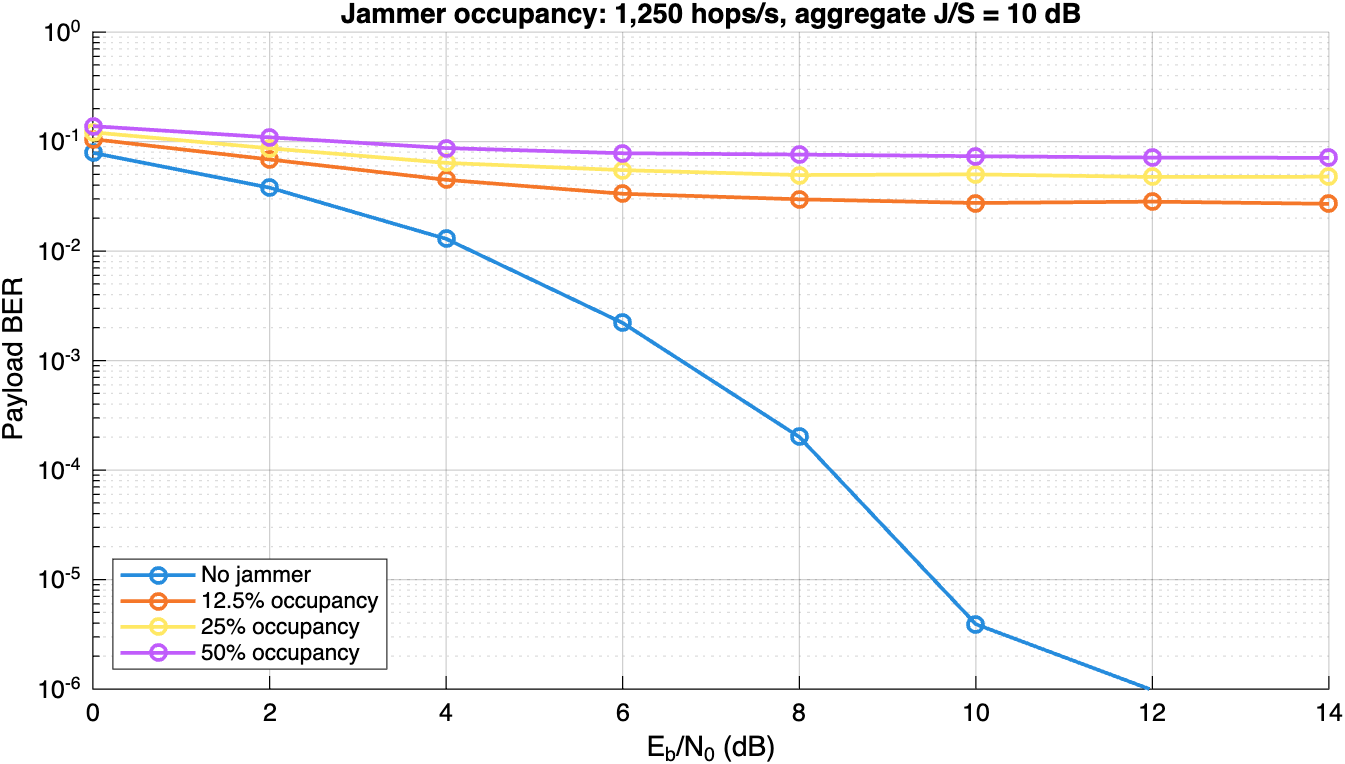
\includegraphics[width=0.85\linewidth,height=\textheight,keepaspectratio,alt={Figure
D1. Payload BER against E\_b/N\_0 at 1,250 hops/s for four jammer
occupancies. Aggregate J/S=10 dB for the jammer
cases.}]{figures/D1_occupancy.png}
\caption{Figure D1. Payload BER against \(E_b/N_0\) at 1,250 hops/s for
four jammer occupancies. Aggregate \(J/S=10\) dB for the jammer cases.}
\end{figure}

Without a jammer, BER decreases rapidly as \(E_b/N_0\) increases. The
measured curve agrees with the expected behaviour of coherent BPSK in
AWGN.

With a jammer, the curves flatten at high \(E_b/N_0\). For example, at
25\% occupancy, BER is approximately 0.0638 at 4 dB, 0.0501 at 10 dB and
0.0477 at 14 dB. Increasing \(E_b/N_0\) reduces ordinary noise errors,
but the jammer continues to corrupt the occupied hops. This residual BER
is called an error floor.

PER is more severe than BER. All 250 packets failed at each
nonzero-jammer operating point in the main sweep. One detected error in
a CRC-protected field can reject the entire packet. Hence, a BER of only
a few percent can still produce almost complete packet loss.

An observed PER of 1 is a finite simulation result, not proof that the
true error probability is exactly one. For 250 failures in 250 trials,
the 95\% Wilson interval is approximately 0.985 to 1.

The main occupancy sweep supplies the correct packet timing to the
receiver. Therefore, this graph measures the aligned link;
unknown-timing acquisition is considered separately.

\subsection{2. Effect of hop-rate
mismatch}\label{effect-of-hop-rate-mismatch}

The transmitter and receiver must change channels at matching times. Let
the nominal dwell time be \(T_d\). In the mismatch experiment, receiver
dwell time is

\[T_{d,\mathrm{rx}}=T_d(1+\epsilon),\]

where \(\epsilon\) is the fractional dwell-duration error. A positive
error makes the receiver dwell longer and hop more slowly. A negative
error makes it hop faster.

After \(H\) hops, the approximate boundary drift is

\[\Delta t\approx H\epsilon T_d.\]

Even a small error accumulates across a frame. The receiver eventually
listens on a different frequency from the transmitter, causing incorrect
BPSK decisions.

\begin{figure}
\centering
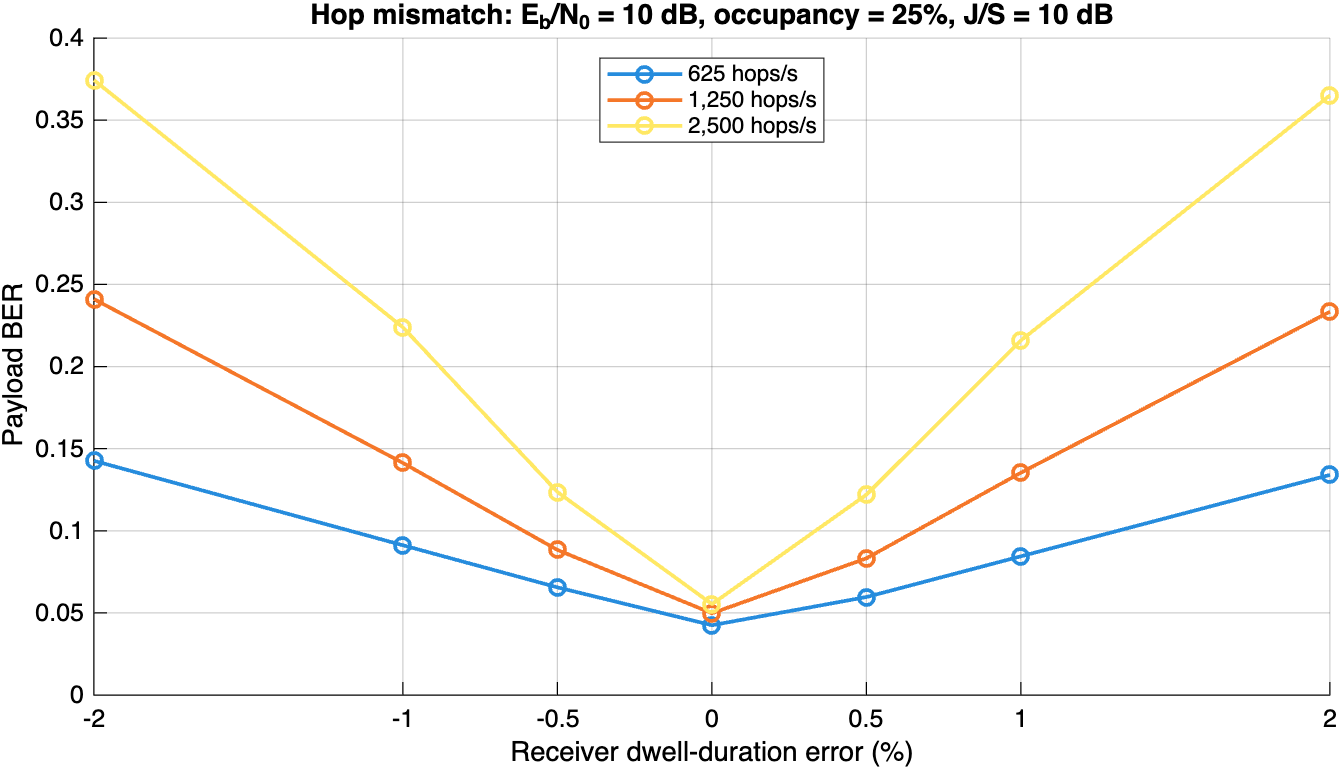
\includegraphics[width=0.85\linewidth,height=\textheight,keepaspectratio,alt={Figure
D2. BER against receiver dwell-duration error for three hop rates, at
E\_b/N\_0=10 dB, 25\% occupancy and J/S=10
dB.}]{figures/D2_mismatch.png}
\caption{Figure D2. BER against receiver dwell-duration error for three
hop rates, at \(E_b/N_0=10\) dB, 25\% occupancy and \(J/S=10\) dB.}
\end{figure}

\begin{minipage}{\linewidth}

{\def\LTcaptype{none} % do not increment counter
\begin{longtable}[]{@{}
  >{\raggedleft\arraybackslash}p{(\linewidth - 6\tabcolsep) * \real{0.2500}}
  >{\raggedleft\arraybackslash}p{(\linewidth - 6\tabcolsep) * \real{0.2500}}
  >{\raggedleft\arraybackslash}p{(\linewidth - 6\tabcolsep) * \real{0.2500}}
  >{\raggedleft\arraybackslash}p{(\linewidth - 6\tabcolsep) * \real{0.2500}}@{}}
\toprule\noalign{}
\begin{minipage}[b]{\linewidth}\raggedleft
Dwell error
\end{minipage} & \begin{minipage}[b]{\linewidth}\raggedleft
BER at 625 hops/s
\end{minipage} & \begin{minipage}[b]{\linewidth}\raggedleft
BER at 1,250 hops/s
\end{minipage} & \begin{minipage}[b]{\linewidth}\raggedleft
BER at 2,500 hops/s
\end{minipage} \\
\midrule\noalign{}
\endhead
\bottomrule\noalign{}
\endlastfoot
-2\% & 0.1426 & 0.2410 & 0.3744 \\
-1\% & 0.0912 & 0.1413 & 0.2238 \\
0\% & 0.0425 & 0.0498 & 0.0553 \\
+1\% & 0.0845 & 0.1354 & 0.2159 \\
+2\% & 0.1340 & 0.2334 & 0.3651 \\
\end{longtable}
}

\end{minipage}

Each curve has its minimum near zero mismatch. Faster hopping is more
sensitive to the same fractional dwell error because the accumulated
drift covers a larger fraction of a short dwell.

For example, a frame lasts 32 ms. At 1\% dwell error, boundary drift is
approximately 0.32 ms. This is about 20\%, 40\% and 80\% of one dwell at
625, 1,250 and 2,500 hops/s respectively. The calculation explains why
the fastest rate shows the largest BER increase.

PER remains 1 throughout this mismatch study because the existing jammer
already causes every tested packet to fail. Therefore, BER is the more
useful measure for showing the additional damage caused by mismatch. The
results do not show a further PER increase above one.

A wrong hopping-code position also causes severe degradation. A forced
one-hop offset gives BER values of approximately 0.503, 0.498 and 0.487
at the three rates, close to random binary decisions. Correct
hopping-code alignment is therefore essential.

\subsection{3. FHSS and fixed-frequency
comparison}\label{fhss-and-fixed-frequency-comparison}

The comparison uses the same BPSK symbol rate and average transmitted
power. Four cases are studied: FHSS, a fixed carrier inside the jammed
band, a fixed carrier outside it, and a fixed channel chosen uniformly
at random for each packet.

This comparison uses the idealized symbol model with perfect channel
isolation. It supports a relative comparison but should not be
numerically mixed with the waveform results in Figures D1 and D2.

\begin{figure}
\centering
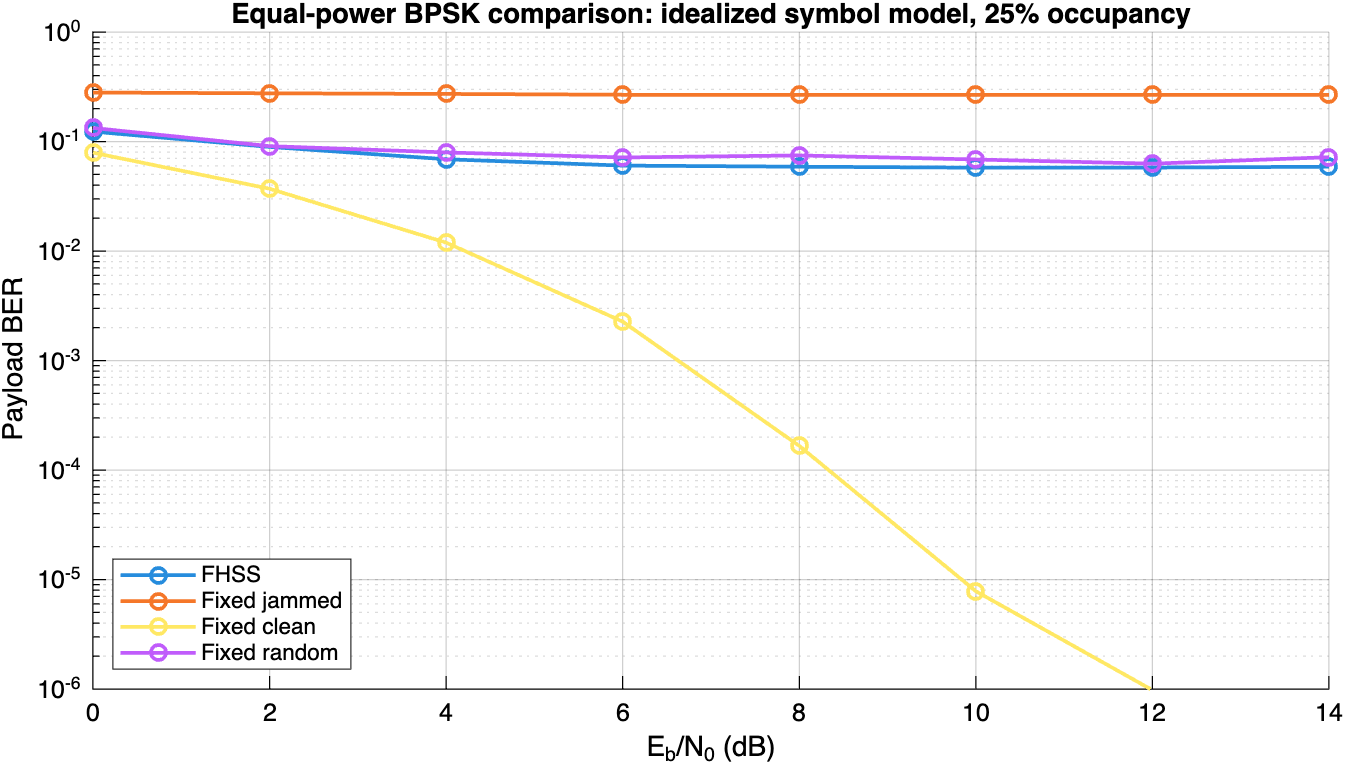
\includegraphics[width=0.85\linewidth,height=\textheight,keepaspectratio,alt={Figure
D3. Equal-power BPSK comparison using the idealized symbol model. Jammer
occupancy is 25\%, aggregate J/S=10 dB, and FHSS uses 1,250
hops/s.}]{figures/D3_fixed_link.png}
\caption{Figure D3. Equal-power BPSK comparison using the idealized
symbol model. Jammer occupancy is 25\%, aggregate \(J/S=10\) dB, and
FHSS uses 1,250 hops/s.}
\end{figure}

At \(E_b/N_0=10\) dB:

{\def\LTcaptype{none} % do not increment counter
\begin{longtable}[]{@{}lrr@{}}
\toprule\noalign{}
Link & Payload BER & PER \\
\midrule\noalign{}
\endhead
\bottomrule\noalign{}
\endlastfoot
FHSS & 0.05769 & 1 \\
Fixed jammed carrier & 0.26614 & 1 \\
Fixed clean carrier & \(7.813\times10^{-6}\) & 0.002 \\
Random fixed channel per packet & 0.06850 & 0.2591 \\
\end{longtable}
}

The fixed jammed link performs worst in BER because it remains inside
the interference continuously. FHSS leaves the jammed channels and sends
part of the message through clear channels. Its average BER is therefore
much lower than that of the permanently jammed fixed link.

A guaranteed clean fixed channel gives the best result because it avoids
the jammer completely. However, this assumes that a clean channel is
known and remains available.

The random fixed-channel link has similar average BER to FHSS but much
lower PER in this experiment. At 25\% occupancy, approximately one
quarter of packets choose a jammed carrier, while the others use clean
carriers. FHSS distributes jammed symbols across almost every frame, so
CRC can reject every frame even when its average BER is lower.

Thus, FHSS improves resistance to remaining on one jammed frequency, but
does not guarantee lower PER than every fixed-frequency strategy.
Without error correction or retransmission, the present jammer is too
strong for reliable delivery of complete FHSS packets.

\subsection{4. Validation of the
results}\label{validation-of-the-results}

Without interference, coherent BPSK should follow

\[P_b=\frac{1}{2}\operatorname{erfc}\left(\sqrt{E_b/N_0}\right).\]

At 4 dB and 1,250 hops/s, the measured BER is approximately 0.0129
against a theoretical value of 0.0125. At 10 dB, two payload errors in
512,000 tested bits give \(3.906\times10^{-6}\), close to the
theoretical \(3.872\times10^{-6}\). These values support the AWGN
scaling used in Part B.

Noiseless synchronized tests recover the exact payload at every hop
rate. CRC-16 produces the reference value \texttt{0x29B1} for
\texttt{123456789}. Seeded hopping is repeatable and visits all eight
channels once in each complete permutation block.

\subsection{5. Engineering
recommendation}\label{engineering-recommendation}

\subsubsection{Hop-set size and
bandwidth}\label{hop-set-size-and-bandwidth}

The symbol rate is \(R_s=10\) ksymbol/s. Rectangular BPSK has an
approximate first-null bandwidth of

\[B_{\mathrm{ch}}\approx2R_s=20\ \mathrm{kHz}.\]

For channel spacing \(\Delta f=25\) kHz and available hopping span 195
kHz,

\[B_{\mathrm{hop}}=(N-1)\Delta f+B_{\mathrm{ch}}.\]

Therefore,

\[N\leq1+\frac{195-20}{25}=8.\]

The recommended hop set is eight channels. This uses the available
main-lobe bandwidth and spreads transmission across the whole assigned
band. The 195 kHz value is a first-null span estimate, not a strict
limit on all radiated energy; rectangular pulses have sidelobes.

\subsubsection{Hop rate}\label{hop-rate}

With eight symbols per hop,

\[T_d=\frac{8}{10,000}=0.8\ \mathrm{ms},\qquad R_h=\frac{1}{T_d}=1,250\ \mathrm{hops/s}.\]

The recorded acquisition success probabilities at 10 dB and 25\%
occupancy are:

{\def\LTcaptype{none} % do not increment counter
\begin{longtable}[]{@{}rrr@{}}
\toprule\noalign{}
Hop rate & Acquisition success & Dwell time \\
\midrule\noalign{}
\endhead
\bottomrule\noalign{}
\endlastfoot
625 hops/s & 50\% & 1.6 ms \\
1,250 hops/s & 92\% & 0.8 ms \\
2,500 hops/s & 90\% & 0.4 ms \\
\end{longtable}
}

Each value is based on 50 acquisition trials. The two faster rates are
within five percentage points of the best observed acquisition
performance. Their PER results under strong jamming do not establish a
delivery advantage for 2,500 hops/s. Therefore, choose the slower
eligible rate, 1,250 hops/s, to reduce switching demands and sensitivity
to dwell mismatch.

The recommendation is a practical choice among the tested settings,
rather than proof of a universally optimal hop rate.

\subsection{Conclusion}\label{conclusion}

Increasing jammer occupancy raises BER in the tested channel, and
interference creates an error floor at high \(E_b/N_0\). Receiver dwell
mismatch causes accumulated timing drift, with faster hopping showing
greater sensitivity. FHSS has lower BER than a fixed link trapped on a
jammed carrier, although a known clean fixed carrier performs better.
The recommended configuration is eight channels over a nominal 195 kHz
span at 1,250 hops/s, with 0.8 ms dwell time. Error correction,
retransmission, or interference-aware channel selection would be needed
to improve complete-packet delivery under the strong jammer used here.

\end{document}
